\section{Implementation Approach}
\label{section:impl}
Clouds are comprehensible indicators for telling the weather. 
They offer many visible features to make an rough prediction of the weather conditions, or weather changes to come.
As described in \sectionref{section:clouds:types}, some cloud types only form under specific conditions.
Also, whenever certain clouds are present, \gls{precipitation} is shortly followed, as it is with altostratus clouds.
\\
Those factors allow a prediction of the weather, but for this project, the process is reversed.
The given data is not an image of clouds, but meteorological measurement data, and the desired outcome is not a prediction, but an image of clouds.

\begin{figure}[H]
    \centering
    \begin{minipage}{0.47\linewidth}
        \begin{tikzpicture}
            \tikzset{edge/.style = {-{Latex[length=3mm]},shorten >= -4pt}}
            \tikzset{shortedge/.style = {shorten <=-4pt,shorten >= -4pt}}
            \tikzset{shortshortedge/.style = {shorten <=-5.5pt,shorten >= -5.3pt}}
            \tikzset{shortshortedge2/.style = {shorten <=-4.5pt,shorten >= -4.5pt}}

            % rainy clouds
            \node (cloud1) at (0.5, 2.0) {};
            \node (cloud2) at (0.8, 2.2) {};
            \node (cloud5) at (1.6, 2.0) {};
            \node (cloud3) at (1.0, 1.9) {};
            \node (cloud4) at (1.3, 2.2) {};
            \node[cloud,fill=gray!30,cloud puffs=9, cloud, minimum width=0.5cm, minimum height=0.2cm, align=center, draw] (cloud) at (cloud1) {};
            \node[cloud,fill=gray!30,cloud puffs=9, cloud, minimum width=0.5cm, minimum height=0.2cm, align=center, draw] (cloud) at (cloud2) {};
            \node[cloud,fill=gray!30,cloud puffs=9, cloud, minimum width=0.5cm, minimum height=0.2cm, align=center, draw] (cloud) at (cloud5) {};
            \node[cloud,fill=gray!30,cloud puffs=12, cloud, minimum width=1.0cm, minimum height=0.7cm, align=center, draw] (cloud) at (cloud3) {};
            \node[cloud,fill=gray!30,cloud puffs=12, cloud, minimum width=0.8cm, minimum height=0.5cm, align=center, draw] (cloud) at (cloud4) {};
            \draw[edge] (2.5, 2) -- (3.5,2);
            \node[anchor=west,font=\small] at (4,2) {rain ahead};

            % clear clouds
            \node (cloud1) at (0.5, 0.0) {};
            \node (cloud2) at (0.9, 0.2) {};
            \node (cloud5) at (1.6, 0.0) {};
            \node[cloud,fill=white,cloud puffs=9, cloud, minimum width=0.5cm, minimum height=0.2cm, align=center, draw] (cloud) at (cloud1) {};
            \node[cloud,fill=white,cloud puffs=9, cloud, minimum width=0.5cm, minimum height=0.2cm, align=center, draw] (cloud) at (cloud2) {};
            \node[cloud,fill=white,cloud puffs=9, cloud, minimum width=0.5cm, minimum height=0.2cm, align=center, draw] (cloud) at (cloud5) {};
            \draw[edge] (2.5, 0) -- (3.5,0);
            \node[anchor=west,font=\small] at (4,0) {fair weather ahead};

        \end{tikzpicture}
        \captionof{figure}{Weather information based on visual data.}
        \label{img:tikz:impl:data1}
    \end{minipage}        
    \hfill
    \begin{minipage}{0.47\linewidth}
        \begin{tikzpicture}
            \tikzset{edge/.style = {-{Latex[length=3mm]},shorten >= -4pt}}
            \tikzset{shortedge/.style = {shorten <=-4pt,shorten >= -4pt}}
            \tikzset{shortshortedge/.style = {shorten <=-5.5pt,shorten >= -5.3pt}}
            \tikzset{shortshortedge2/.style = {shorten <=-4.5pt,shorten >= -4.5pt}}

            % rainy clouds
            \node (cloud1) at (4.5, 2.0) {};
            \node (cloud2) at (4.8, 2.2) {};
            \node (cloud5) at (5.6, 2.0) {};
            \node (cloud3) at (5.0, 1.9) {};
            \node (cloud4) at (5.3, 2.2) {};
            \node[cloud,fill=gray!30,cloud puffs=9, cloud, minimum width=0.5cm, minimum height=0.2cm, align=center, draw] (cloud) at (cloud1) {};
            \node[cloud,fill=gray!30,cloud puffs=9, cloud, minimum width=0.5cm, minimum height=0.2cm, align=center, draw] (cloud) at (cloud2) {};
            \node[cloud,fill=gray!30,cloud puffs=9, cloud, minimum width=0.5cm, minimum height=0.2cm, align=center, draw] (cloud) at (cloud5) {};
            \node[cloud,fill=gray!30,cloud puffs=12, cloud, minimum width=1.0cm, minimum height=0.7cm, align=center, draw] (cloud) at (cloud3) {};
            \node[cloud,fill=gray!30,cloud puffs=12, cloud, minimum width=0.8cm, minimum height=0.5cm, align=center, draw] (cloud) at (cloud4) {};
            \draw[edge] (1.2, 2) -- (3.5,2);
            \node[anchor=west,font=\small] at (-1,2) {rain ahead};

            % clear clouds
            \node (cloud1) at (4.5, 0.0) {};
            \node (cloud2) at (4.9, 0.2) {};
            \node (cloud5) at (5.6, 0.0) {};
            \node[cloud,fill=white,cloud puffs=9, cloud, minimum width=0.5cm, minimum height=0.2cm, align=center, draw] (cloud) at (cloud1) {};
            \node[cloud,fill=white,cloud puffs=9, cloud, minimum width=0.5cm, minimum height=0.2cm, align=center, draw] (cloud) at (cloud2) {};
            \node[cloud,fill=white,cloud puffs=9, cloud, minimum width=0.5cm, minimum height=0.2cm, align=center, draw] (cloud) at (cloud5) {};
            \draw[edge] (2.5, 0) -- (3.5,0);
            \node[anchor=west,font=\small] at (-1,0) {fair weather ahead};
            
        \end{tikzpicture}
        \captionof{figure}{Visual construction based on weather information.}
        \label{img:tikz:impl:data2}       
    \end{minipage}
\end{figure}

\noindent
For any given day to render, an implementation would require data from that day but also from the near future of that day.
So, in order to render a cloud image for day $x$, a potential algorithm could look like this.
Note that the listing below describes only an idea and is by no means final or compulsory.

\begin{lstlisting}[language=HLSL, caption=Pseudo-code of cloud render algorithm., label=lst:pseudo:algorithm]
// weather data including 7-day forecast
WeatherData data;
CloudRenderer renderer;

function renderClouds(Day x) {
    if (x > TODAY + 7) throw;

    d1 = data.getDataFor(x);
    d2 = data.getDataFor(x + 1);
    d3 = data.getDataFor(x + 2);
    // and so on...

    // sophisticated checks about current and future conditions:
    if (d1.fairWeather && d2.fairWeather)
        return renderer.clearSky();
    if (d1.fairWeather && d2.isRaining)
        return renderer.cloudsOnclearDayBeforeRain();
    if (d1.isRaining)
        return renderer.cloudsOnRainyDay();
    if (d2.isRaining) 
        return renderer.cloudsBeforeRainyDay();
    if (d3.isRaining) 
        return renderer.clouds2DaysBeforeRainyDay();
    // and so on...
    
}
\end{lstlisting}

\clearpage

\subsection{Look-Ahead Issue}
The approach as described above relies on having data from a couple of days ahead of time. Assumed that number of days is $t$, then the weather data for day $x$ could only be rendered $t$ days after $x$.
That would mean, for such an approach to work, the weather of today can not be rendered before $t$ days later.
\\
In this case however, the weather measurement data retrieved from \emph{meteoblue} also contains a seven-day weather forecast. 
Given that $t$ is less than or equal to seven (days), an implementation cloud still produces accurate cloud imagery.

\subsection{Layers of Cloud Shaders}
\label{section:impl:layers}
As identified in \sectionref{section:clouds:types}, most of the clouds in the troposphere only appear at certain \gls{altitude}s.
The high-level clouds are all of type \emph{cirrus}.
The mid-level types are altostratus and altocumulus, while the low-level types are cumulus, stratocumulus and stratus.
\\
This leads to the conclusion that some of the cloud types could be consolidated into a combined layer and rendered by the same shader.
Exception to that are only the two larger types that span over multiple height levels: nimbostratus and cumulonimbus. For those, a more unique solution has to be found.

\begin{figure}[H]
    \centering
    \begin{tikzpicture}[scale=1]
        \tikzset{edge/.style = {-{Latex[length=3mm]},shorten >= -4pt}}
        \tikzset{shortedge/.style = {shorten <=-4pt,shorten >= -4pt}}
        \tikzset{icon/.style = {font=\Large}}
        \tikzset{mini/.style = {font=\footnotesize}}
        \tikzset{tiny/.style = {font=\tiny}}

        % cloud layer boxes
        \node[inner sep=0pt] at (5.5,5.2) 
            {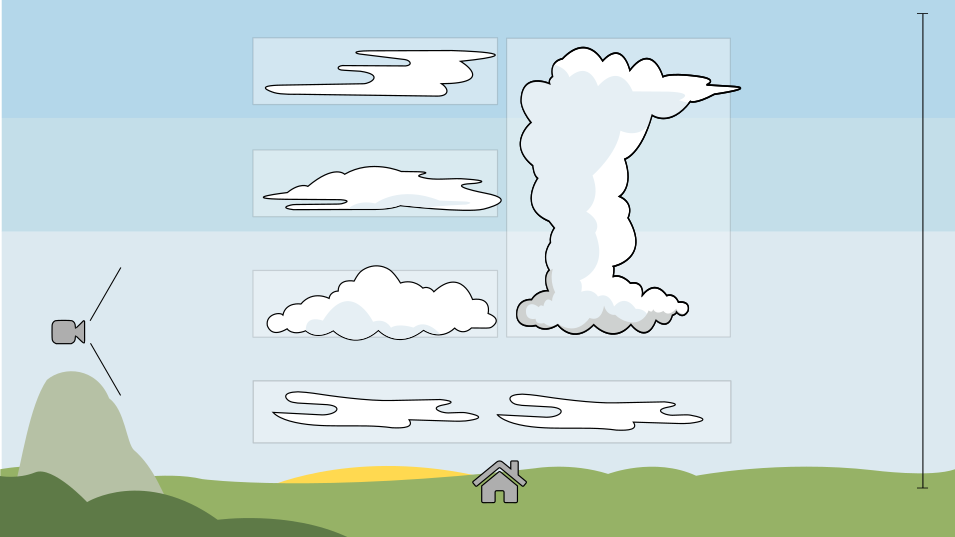
\includegraphics[width=\textwidth]{cloudlayers/cloudlayers.png}};
        \node[right] at (2.85,9.1) {high-level (cirro)};
        \node[right] at (2.85,7.22) {mid-level (alto)};
        \node[right] at (2.85,5.28) {low-level};
        \node[right] at (2.85,3.5) {ground fog};
        \node[right] at (7.0,9.15) {cumulonimbus};

        % other labels
        \node at (-0.3,4.5) {camera};
        \node at (7.0,1.1) {city of Bern};

        % low mid high
        \node[mini,darkdarkcyan] at (-1.6,4.2) {Low};
        \node[mini,darkdarkcyan] at (-1.6,6.7) {Mid};
        \node[mini,darkdarkcyan] at (-1.6,8.5) {High};

        % height numbers
        \node[tiny,darkcyan!60] at (-1.6,5.5) {2000m};
        \node[tiny,darkcyan!80] at (-1.6,7.5) {7000m};
        \node[tiny,darkcyan] at    (-1.6,9.5) {11000m};

    \end{tikzpicture}
    \captionof{figure}{Layers of cloud shaders (adapted from \protect\cite{cloudtypes:wiki}).}
    \label{img:tikz:shadersetup:particles}       
\end{figure}

\pagebreak

\subsubsection{High-Level Clouds}
\label{section:impl:layers:high}
The uppermost layer would contain cirrus, cirrostratus and cirrocumulus clouds.
All of these form under similar weather conditions and closely resemble each other in appearance and formation.
\\
A potential \gls{shader} for that layer could be programmed to render a base variant of all three cirrus clouds, which would then be parametrized into each individual type of cirrus cloud, whichever is currently visible.

\begin{figure}[H]
    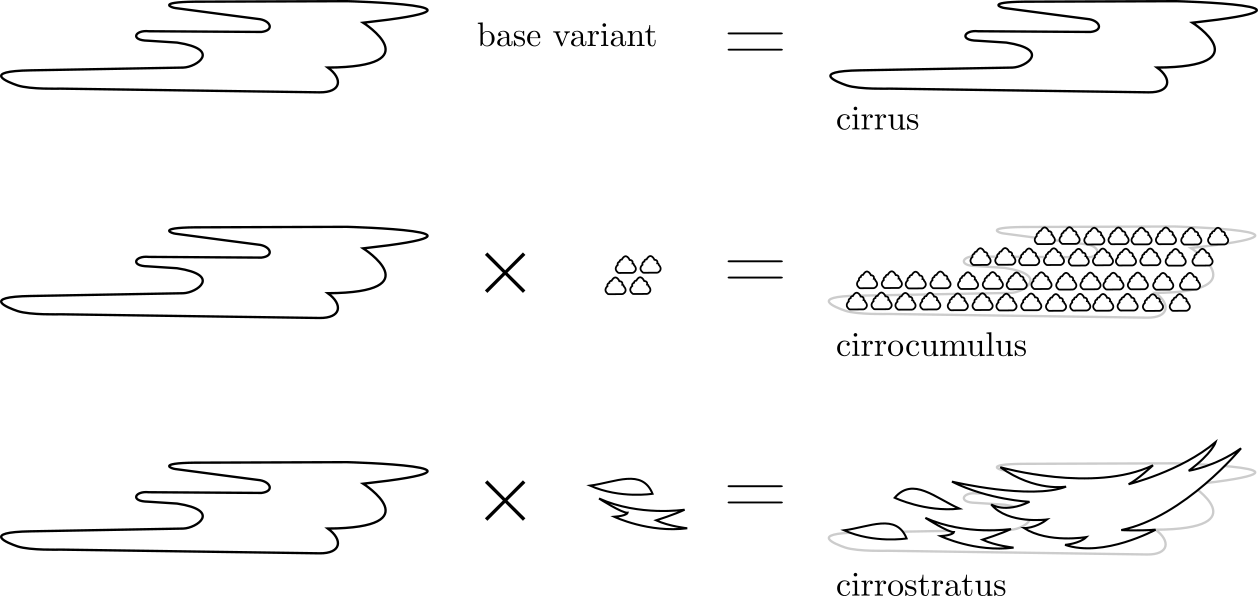
\includegraphics[width=\linewidth]{cloudlayers/cirruslayer.png}
    \caption{Breakdown of the highest shader layer.}
    \label{img:cloudlayer:cirrus}
\end{figure}

\subsubsection{Mid-Level Clouds}
\label{section:impl:layers:mid}
The middle layer consists of altostratus and altocumulus clouds, the latter mainly occurring due to dissipation of the former one.
Since they have many shared characteristics, apart from the puffiness, they are predestined to be processed together.
\\
Given a \gls{shader} is flexible enough to render altostratus clouds, then it is most likely also able to render altocumulus, with only a few adjustments necessary.

\begin{figure}[H]
    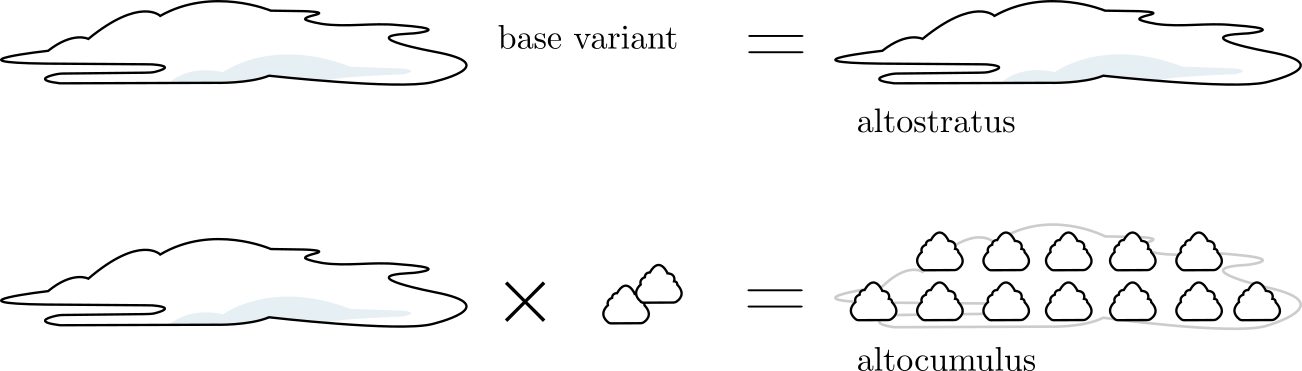
\includegraphics[width=\linewidth]{cloudlayers/altolayer.png}
    \caption{Breakdown of the middle shader layer.}
    \label{img:cloudlayer:alto}
\end{figure}

\pagebreak

\subsubsection{Low-Level Clouds}
\label{section:impl:layers:low}
The lower layer may prove to be more complex than the others, as the stratus and cumulus clouds do essentially not look alike.
However, cumulus clouds could be described as less denser, smaller and separated instances of stratocumulus clouds.
\\
If a \gls{shader} would be able to render stratocumulus clouds and allow to control the density or the spreading of such, then cumulus clouds could be rendered in the same manner.

\begin{figure}[H]
    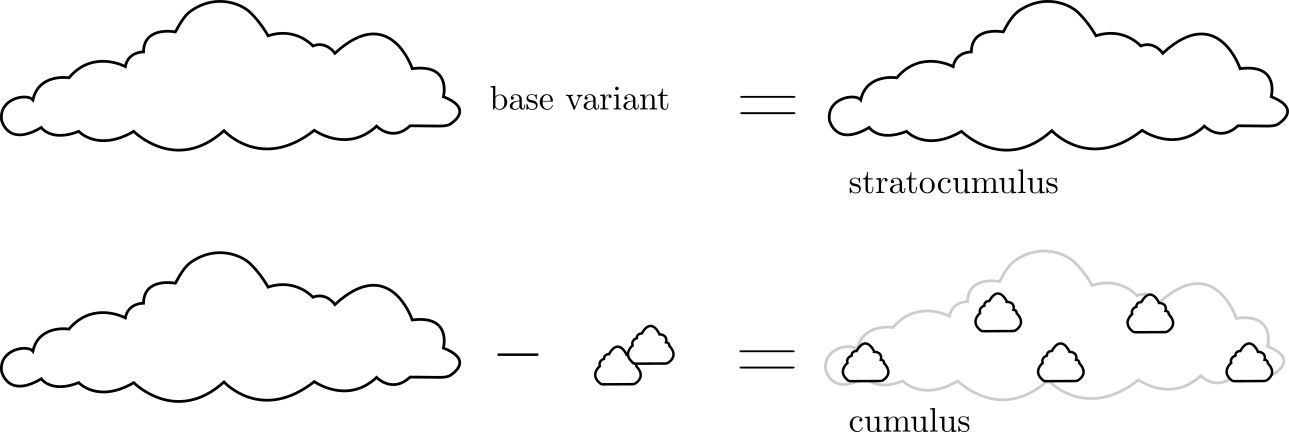
\includegraphics[width=\linewidth]{cloudlayers/stratolayer.png}
    \caption{Breakdown of the lowest shader layer.}
    \label{img:cloudlayer:strato}
\end{figure}


\subsubsection{Ground Level Fog}
\label{section:impl:layers:fog}
The lowest or ground layer consists of fog. It is conceivable that stratus clouds will also be placed in that layer.
Both type of clouds are to some extent combinable, as they primarily vary in density.
\\
Therefore, a \gls{shader} would need to have control over the outcome's density and lightness for it to be able to render both stratus clouds and ground fog.

\begin{figure}[H]
    
\includegraphics[width=\linewidth]{cloudlayers/foglayer.png}
    \caption{Breakdown of the fog shader layer.}
    \label{img:cloudlayer:fog}
\end{figure}

\pagebreak

\subsubsection{Cumulonimbus Layer}
\label{section:impl:layers:cumulonimbus}
With all the previous layers implemented, only the two large cloud types are left, one of them is the cumulonimbus.
\\
Assuming the observer is walking directly underneath a cumulonimbus cloud, the cloud itself and its defining visual features are not really recognizable.
It could easily be mistaken for other clouds that produce \gls{precipitation}.

\begin{figure}[H]
    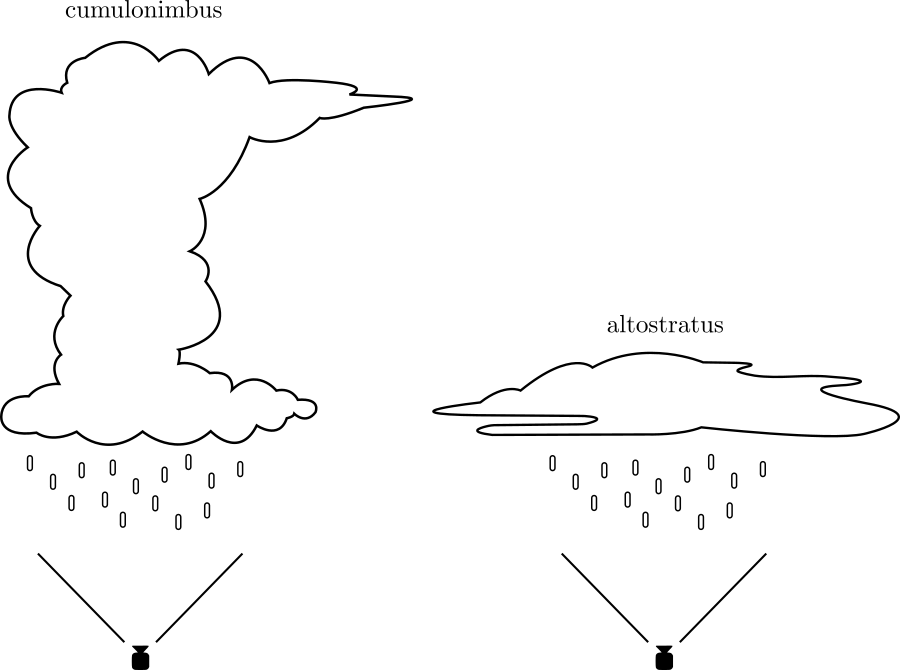
\includegraphics[width=\linewidth]{cloudlayers/cumulonimbus.png}
    \caption{Perspective similarities under clouds with \gls{precipitation}.}
    \label{img:cloudlayer:cumulonimbus}
\end{figure}

\noindent
Under that assumption, it is considered that the cumulonimbus cloud will only ever be seen from a distance.
This is why these clouds will be rendered in their own layer, farther away from the main camera, but spanning over all other height levels.

\pagebreak

\subsubsection{Nimbostratus Substitute}
A similar issue as with the cumulonimbus clouds is present for the nimbostratus clouds.
Due to them being thick, dark layers of cloud lacking features and contours, they are more difficult to render.
\\
It is, however, imaginable to omit the type nimbostratus altogether and substitute it by combining and tuning the already existing layers.
For example, the nimbostratus cloud might be imitated by darkening the color of altostratus clouds as well making them thicker. 
With additional stratus clouds and increased fog density, a layman could probably no longer tell the difference.

\begin{figure}[H]
    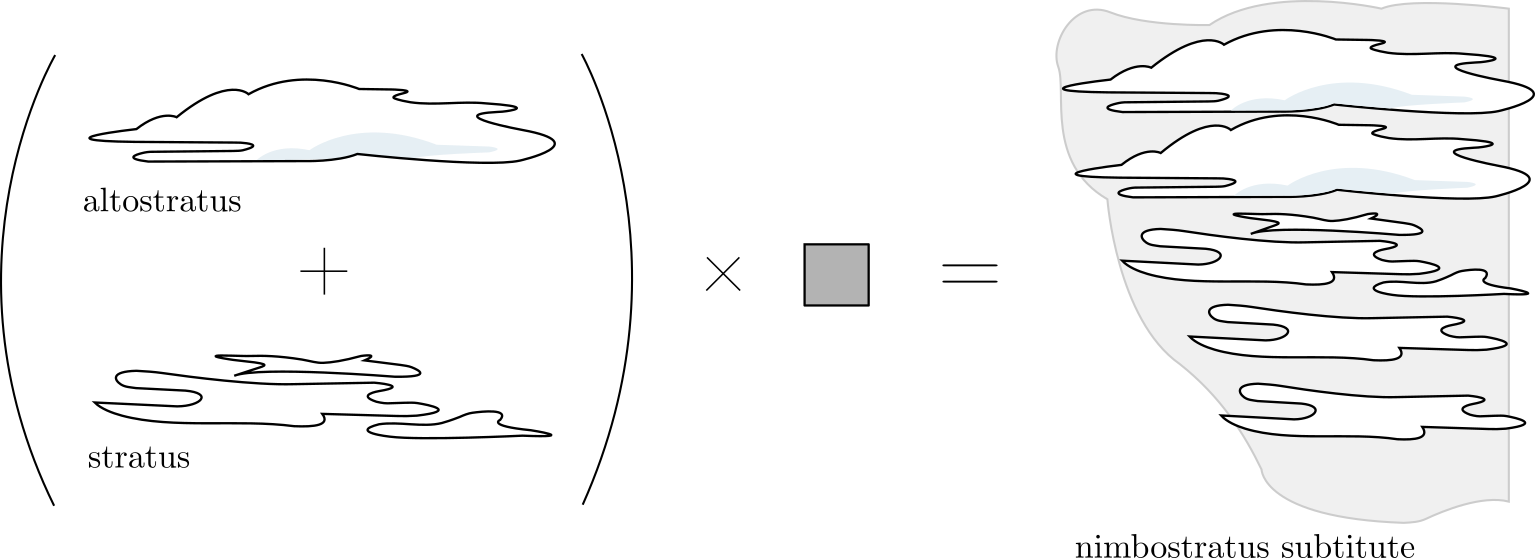
\includegraphics[width=\linewidth]{cloudlayers/nimbostratus.png}
    \caption{Breakdown of the nimbostratus substitute.}
    \label{img:cloudlayer:nimbostratus}
\end{figure}

\subsection{Exclusiveness Issue}
All \gls{shader} layers described in \sectionref{section:impl:layers}, except the cumulonimbus layer, come with an issue.
Given that multiple cloud types are consolidated into one layer, and that layer can only render one cloud type at a time, then no two cloud types of the same layer can ever be rendered together.
\\
However, this rendering system will be a visual representation and not a physically accurate simulation.
Thus, the fact that multiple clouds of the same layer could coexist at the same time, is considered to be negligible and the issue is disregarded in this project.

\pagebreak

\subsection{Background Weather Consideration}
Clouds can be seen from great distances, especially when the observer is located on elevated terrain, which is the case in this project.
For this reason, clouds in close proximity to the observer do not have to be alike more distant ones.
This is also true for weather conditions.
Because of this, whenever rendering cloudscapes from an angle where the horizon is also visible, the weather measurements from places in the far distance also have to be taken into account.
\\
As mentioned in the bachelor project specification document, there are two points of view from which the weather will be rendered.
These are two mountains near the city of Bern: the \emph{Bantiger} and the \emph{Gurten} mountain.
\\
From both peaks, Bern lies in the center of the view. However, a city in the background of each perspective has been chosen to account for weather in the distance.

\begin{figure}[H]
    \centering
        \begin{minipage}{0.47\linewidth}
            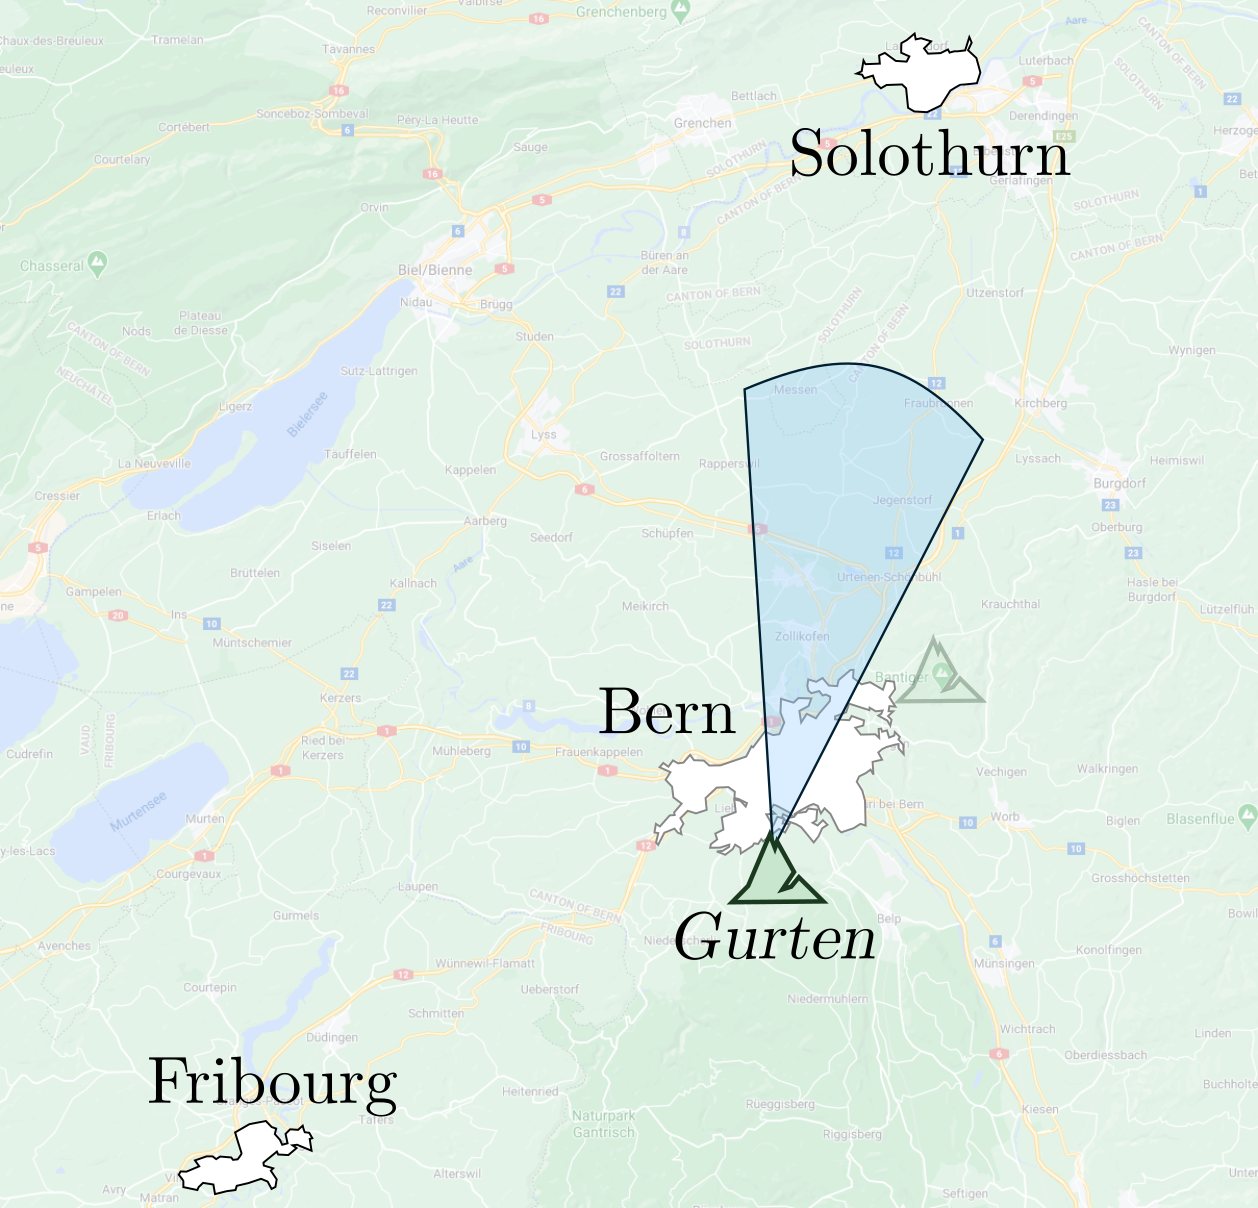
\includegraphics[width=\linewidth]{perspective-gurten.png}
            \captionof{figure}{Perspective view from the Gurten mountain: distant weather in Solothurn is considered.}
            \label{img:noise:fbm10_1}
        \end{minipage}
    \hfill
        \begin{minipage}{0.47\linewidth}
            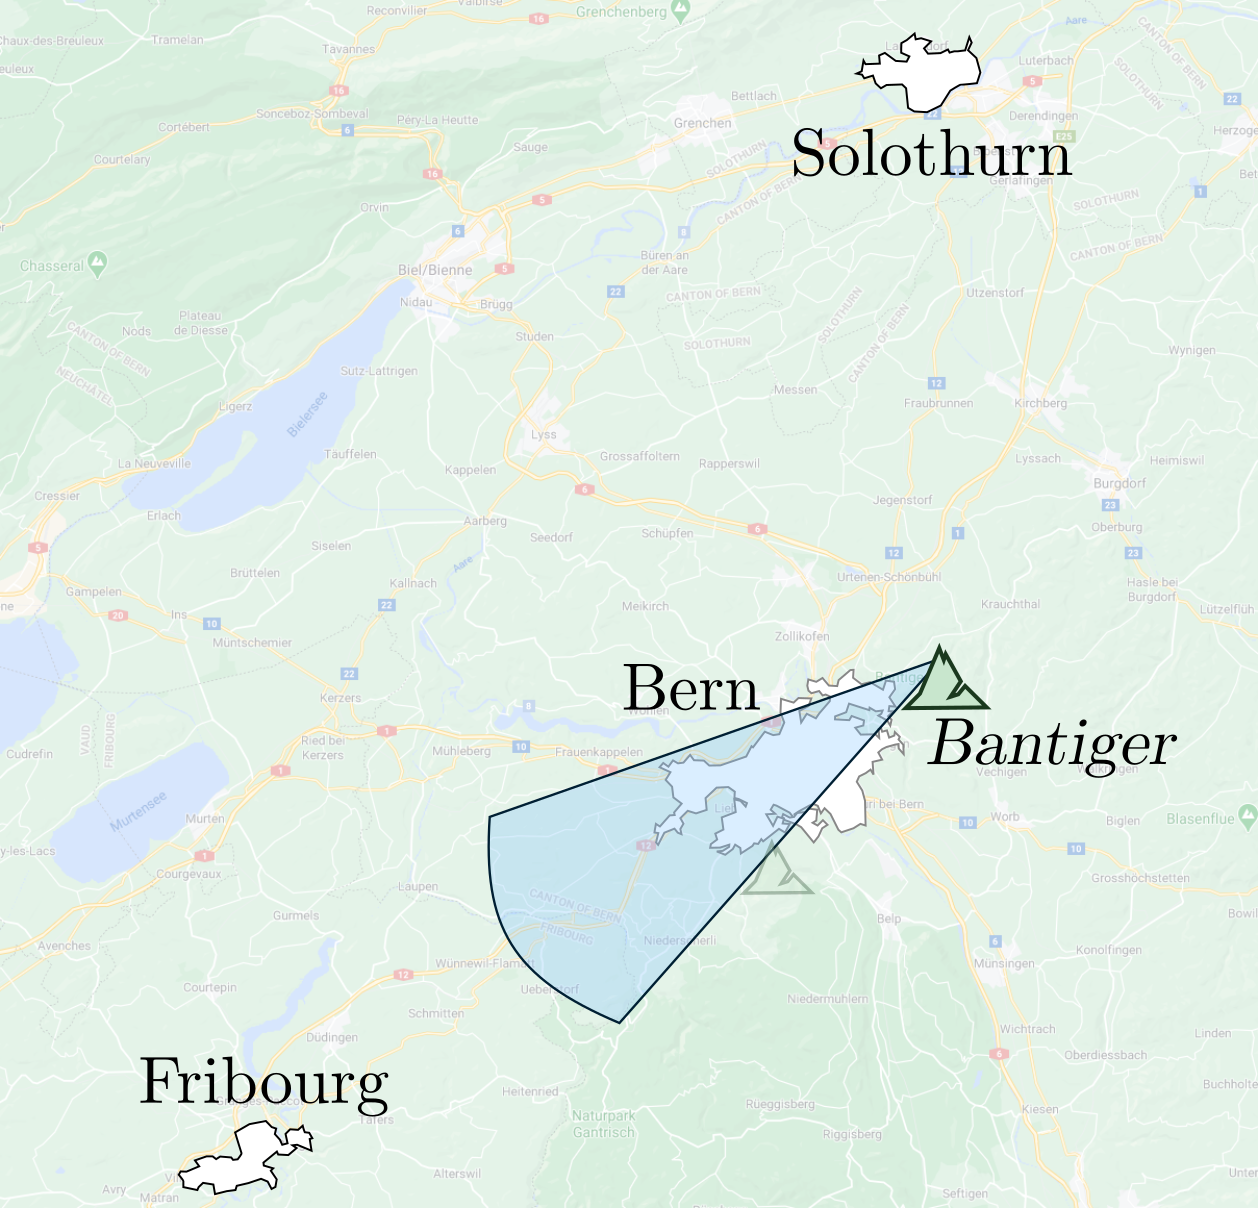
\includegraphics[width=\linewidth]{perspective-bantiger.png}
            \captionof{figure}{Perspective view from the Bantiger mountain: distant weather in Fribourg is considered.}
            \label{img:noise:fbm10_2}
        \end{minipage}
\end{figure}

\pagebreak

\subsection{Weather Data Interpolation}
\label{section:impl:layerinterpolation}
Following up on the background weather consideration, all \gls{shader} layers also need to know those distances and adjust accordingly.
Given there are two measurement sets, one for each city, then the weather in-between can be a combination of both sets.
A very common method to achieve such an evaluation of interim data is called \emph{\gls{lerp}} (lerp).
\Gls{lerp} can be defined as a function $lerp$, if $0 >= t >= 1$: 

$$lerp(a, b, t) = a + (b - a) * t$$

\noindent
Assuming that the two weather measurement sets $w_1$ and $w_2$ can be interpolated, then the function $lerp$ can be used.
In the following example, $w_1$ represents fair weather in Bern, whereas $w_2$ represents cloudy and gloomy weather in Solothurn.
With increasing distance along the axis \color{darkercyan}$L$\color{black}, factor $t$ gradually rises from $0$ to $1$.

\begin{figure}[H]
    \centering
    \begin{tikzpicture}[scale=1]
        \tikzset{edge/.style = {-{Latex[length=3mm]},shorten >= -4pt}}
        \tikzset{shortedge/.style = {shorten <=-4pt,shorten >= -4pt}}
        \tikzset{icon/.style = {font=\Large}}
        \tikzset{mini/.style = {font=\footnotesize}}
        \tikzset{tiny/.style = {font=\tiny}}

        % cloud layer boxes
        \node[inner sep=0pt] at (6.0,4.9) 
            {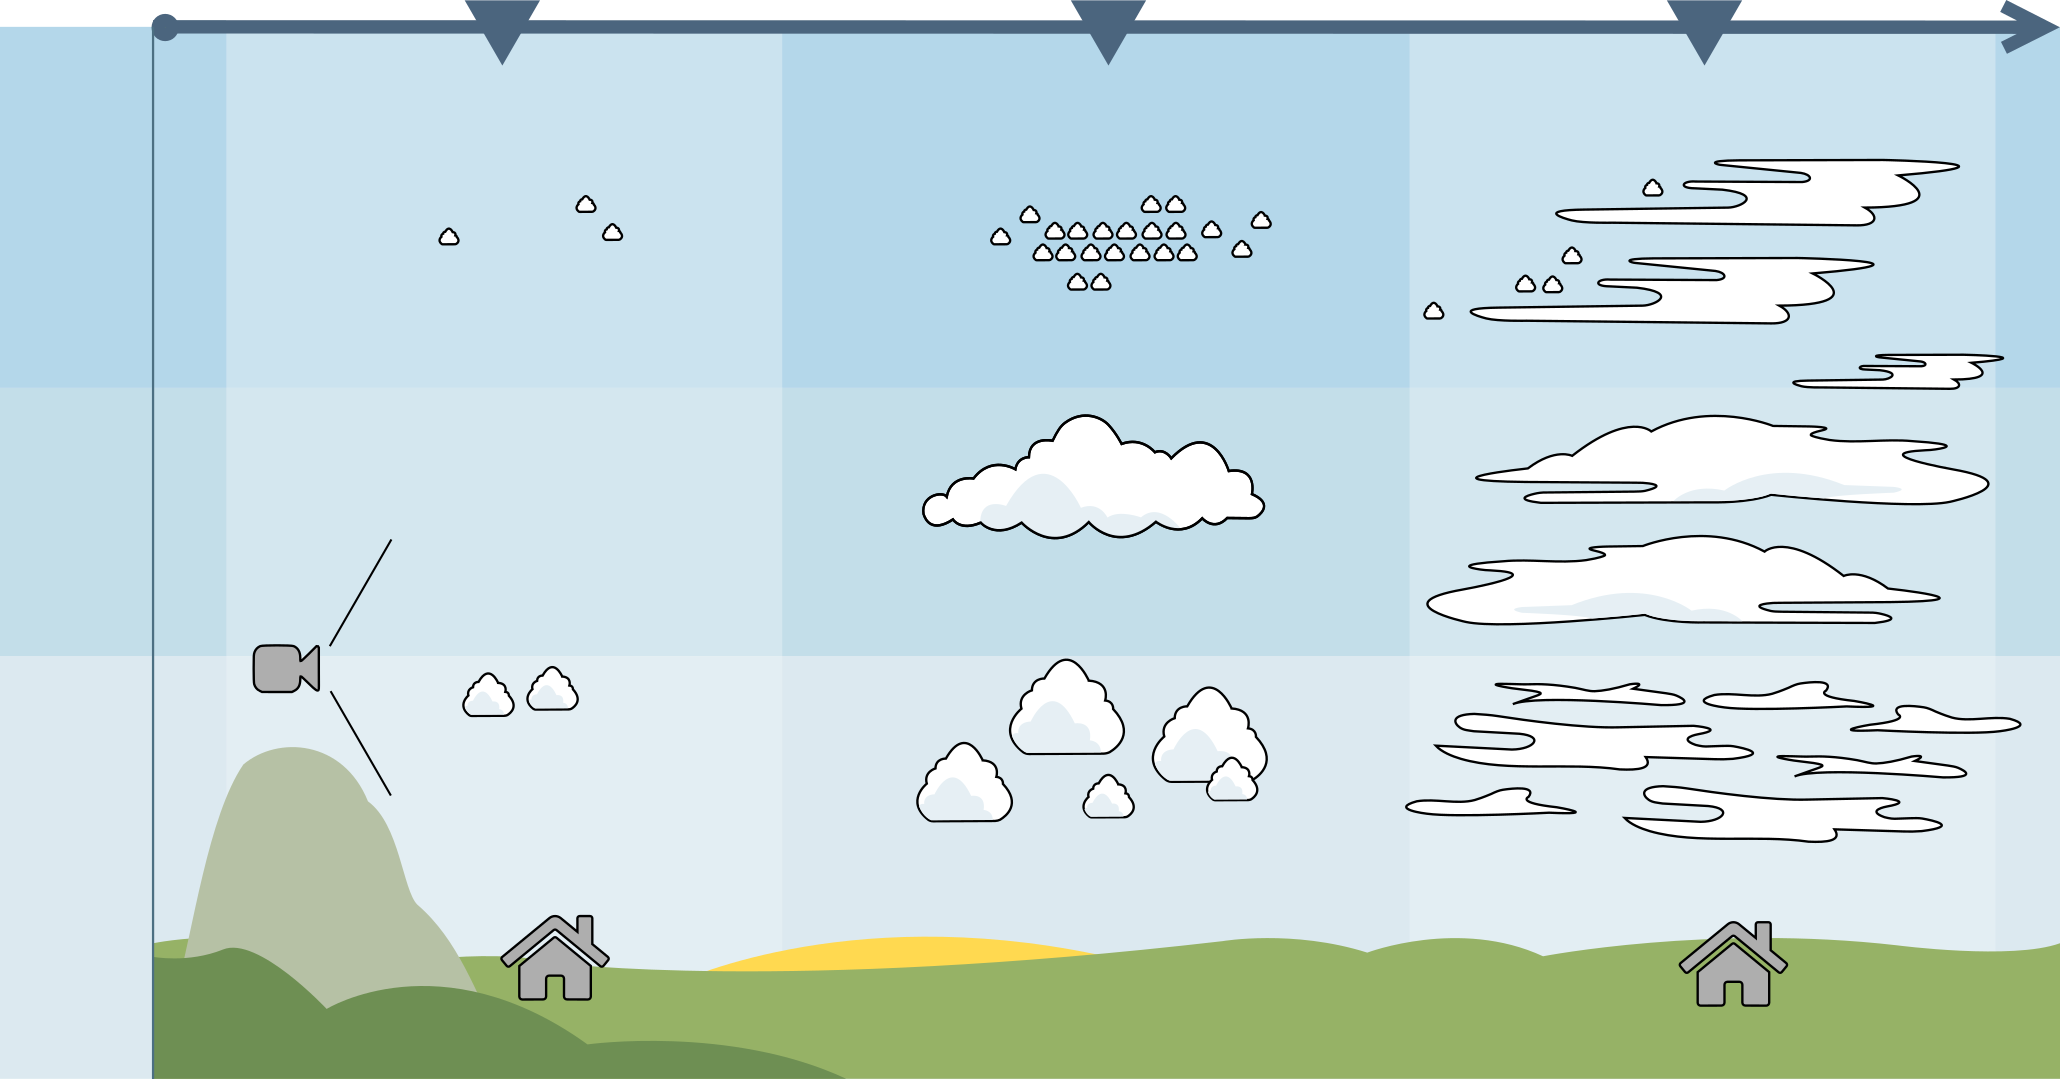
\includegraphics[width=\textwidth]{layer-interpolation.png}};

        % interpolation labels
        \node at (1.9,9.3) {lerp($w_1$,$w_2$, 0)};
        \node at (6.7,9.3) {lerp($w_1$,$w_2$, 0.5)};
        \node at (11.2,9.3) {lerp($w_1$,$w_2$, 1)};

        % other labels
        \node[darkercyan] at (-0.4,9.1) {$L$};
        \node at (0.1,4.4) {camera};
        \node at (2.5,1.1) {city of Bern};
        \node at (11.2,1.1) {city of Solothurn};
        
        % low mid high
        \node[mini,darkdarkcyan] at (-1.15,3.0) {Low};
        \node[mini,darkdarkcyan] at (-1.15,4.9) {Mid};
        \node[mini,darkdarkcyan] at (-1.15,7.6) {High};

        % height numbers
        \node[tiny,darkcyan!60] at (-1.15,3.9) {2000m};
        \node[tiny,darkcyan!80] at (-1.15,5.9) {7000m};
        \node[tiny,darkcyan] at    (-1.15,8.6) {11000m};

    \end{tikzpicture}
    \captionof{figure}{Weather data interpolation for the cloud layers from Bern to Solothurn (adapted from \protect\cite{cloudtypes:wiki}).}
    \label{img:tikz:shadersetup:lerp}       
\end{figure}

\noindent
In summary,  at Bern ($t = 0$), weather for data set $w_1$ is displayed, while at Solothurn ($t = 1$), weather for the data set $w_2$ is rendered.
Everything in-between is a mixture of both data sets, relative to which ever is closer.

\subsection{Alternative Approach}
\label{section:impl:altapproach}
Every subsection that describes another feature of the implementation approach increases the complexity of the developing concept,
which is already depending on many ideas and structures to work.
In cases like this it is best to prepare an alternative approach to implementation, that can be pursued should the primary one fail.
\pagebreak
The core concept of this second implementation approach is based on \gls{particlesystem}s.
It still relies on having four major layers with an additional cumulonimbus block. The nimbostratus will also be substituted.
Those layers are almost identical to the layers described in \sectionref{section:impl:layers:high} to \sectionref{section:impl:layers:cumulonimbus}.
\\
However, instead of the layers each being a single \gls{shader}, they are replaced with a \gls{particlesystem} that emits cubes of clouds.
Those cubes are rendered by different \gls{shader}s, depending on which layer they are spawned in.
The highest layer, \color{darkercyan}$P_1$\color{black}, would emit cloud cubes of the cirrus family.
The middle layer, \color{darkercyan}$P_2$\color{black}, is responsible to render alto cloud cubes.
Layer \color{darkercyan}$P_3$ \color{black} would spawn low-level cloud cubes, while the lowest layer, \color{darkercyan}$P_4$\color{black}, would create fog particles.

\begin{figure}[H]
    \centering
    \begin{tikzpicture}[scale=1]
        \tikzset{edge/.style = {-{Latex[length=3mm]},shorten >= -4pt}}
        \tikzset{shortedge/.style = {shorten <=-4pt,shorten >= -4pt}}
        \tikzset{icon/.style = {font=\Large}}
        \tikzset{mini/.style = {font=\footnotesize}}
        \tikzset{tiny/.style = {font=\tiny}}

        % cloud layer boxes
        \node[inner sep=0pt] at (6.0,4.9) 
            {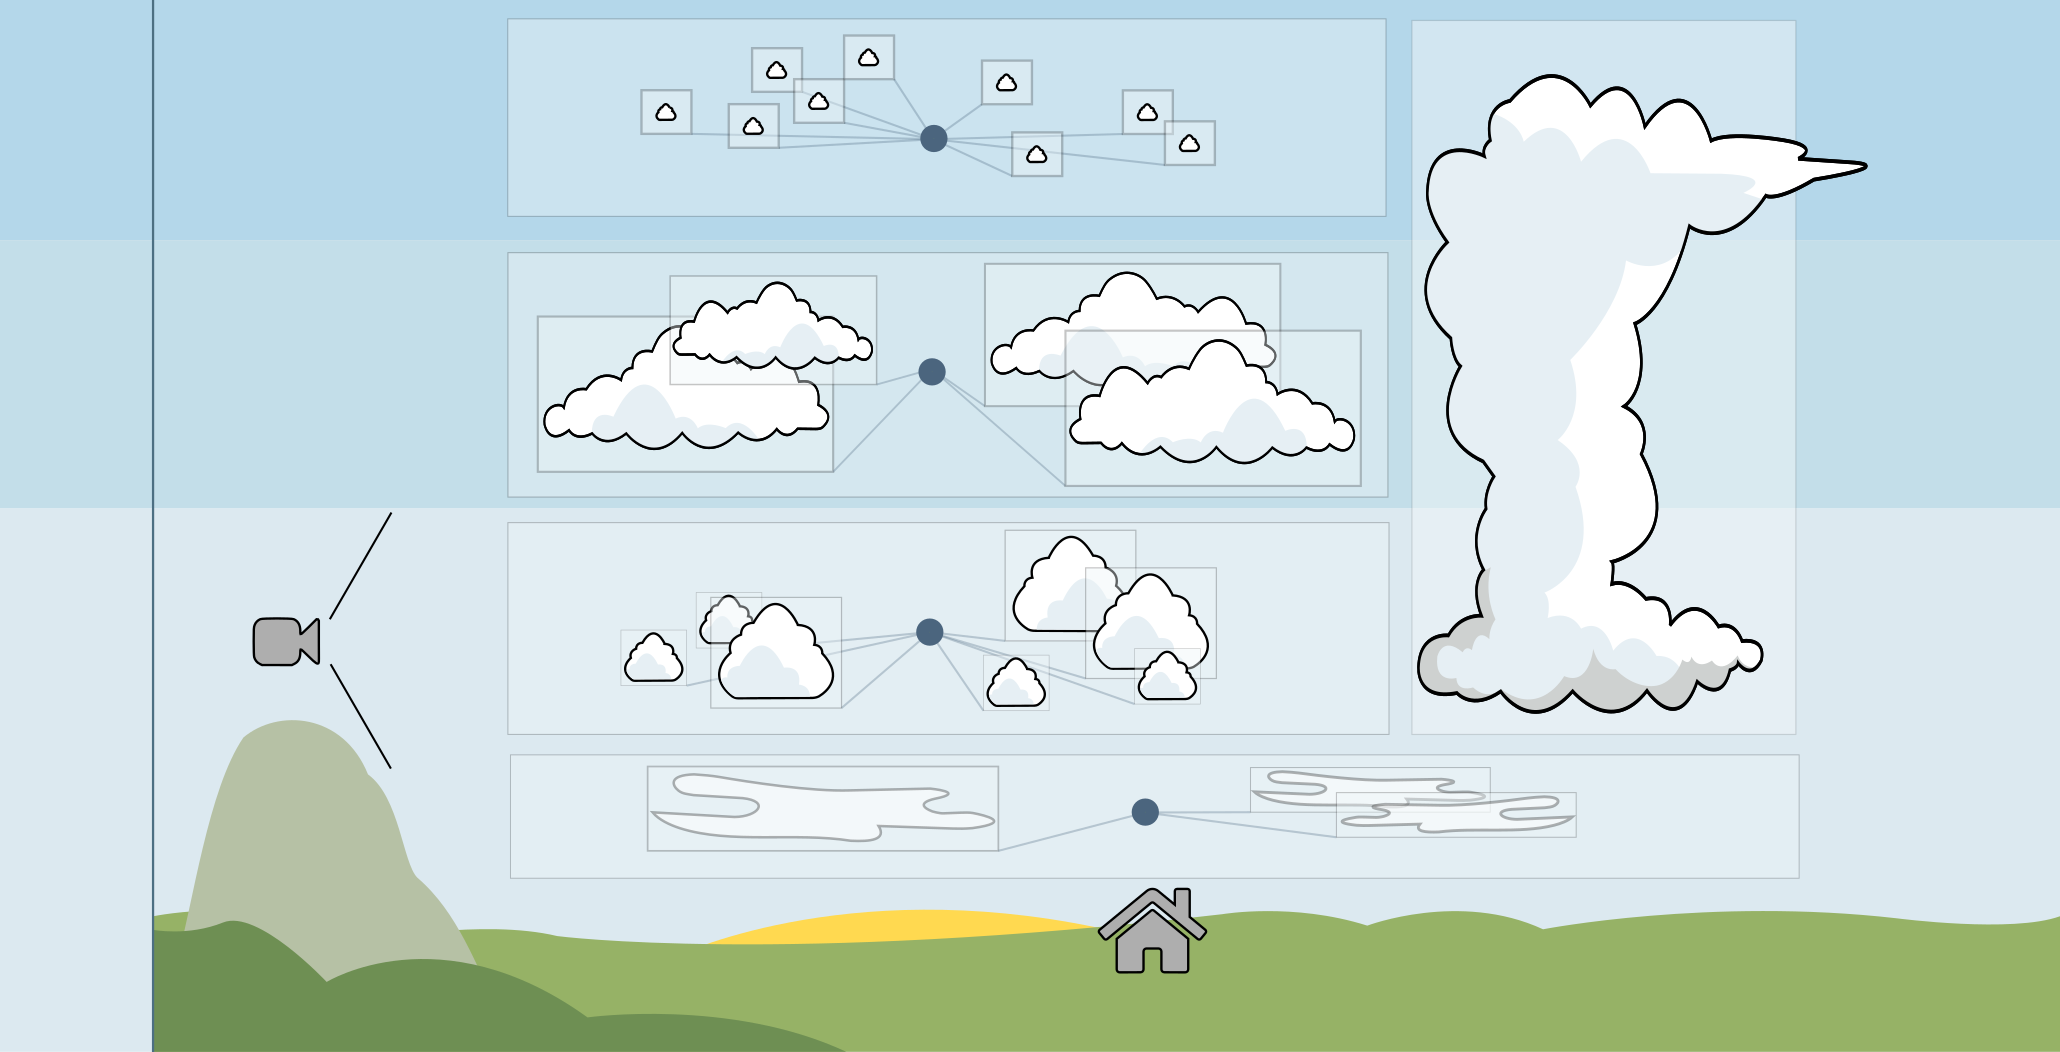
\includegraphics[width=\textwidth]{particlesystem.png}};

        % particle systems
        \node[darkercyan] at (5.0,7.5) {$P_1$};
        \node[darkercyan] at (5.2,6.45) {$P_2$};
        \node[darkercyan] at (5.2,4.5) {$P_3$};
        \node[darkercyan] at (6.5,2.9) {$P_4$};

        % other labels
        \node at (0.1,4.5) {camera};
        \node at (6.9,1.2) {city of Bern};
        
        % low mid high
        \node[mini,darkdarkcyan] at (-1.15,3.3) {Low};
        \node[mini,darkdarkcyan] at (-1.15,6.0) {Mid};
        \node[mini,darkdarkcyan] at (-1.15,7.8) {High};

        % height numbers
        \node[tiny,darkcyan!60] at (-1.15,4.9) {2000m};
        \node[tiny,darkcyan!80] at (-1.15,6.92) {7000m};
        \node[tiny,darkcyan] at    (-1.15,8.65) {11000m};

    \end{tikzpicture}
    \captionof{figure}{Alternative implementation approach based on \gls{particlesystem}s (adapted from \protect\cite{cloudtypes:wiki}).}
    \label{img:tikz:altapproach}       
\end{figure}

\noindent
This alternative approach would offer a much higher flexibility in controlling exactly how many clouds are present.
Each layer is in absolute control of when it spawns cloud particles, how fast the spawn rate is, the particle's size and many more characteristics. 
\\
Nonetheless, contrary to the first approach, a \gls{lerp} of the clouds will prove to be more difficult in this case.
A \gls{particlesystem} cannot be interpolated along two positions, as it is bound to a fixed location.
This issue be could be disregarded at the cost of realism, by only using two \gls{particlesystem}s:
one for Bern and one for the distant city.
Additionally, the number of cloud cubes heavily impacts performance. Should the system be limited regarding the number of cloud cubes, its realism would suffer further.

\subsection{Conclusion}
The implementation approach described in \sectionref{section:impl} will be pursued.
The alternative implementation approach as described in the previous subsection only serves as a backup plan, should a critical problem arise in the first approach.